\section{Dean Module: Student Status Management}

\noindent The Dean Module is for managing the status of students. The Dean has the power to approve a student for a department or cancel their application if there are problems with their records.

\setlength{\fboxsep}{6pt}
\setlength{\fboxrule}{1pt}
\begin{figure}[H]
    \centering
   \fbox{ 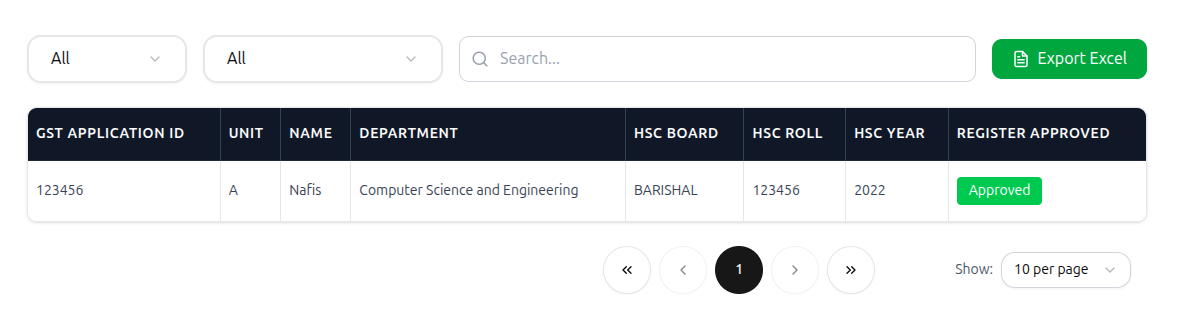
\includegraphics[width=0.8\textwidth]{chapters/chapter4/images/approvedList.png}}
    \caption{Dean’s Portal: Admission Approval and Cancellation Interface}
    \label{fig:dean_status_manage}
\end{figure}

\noindent The Dean can do these things:
\begin{itemize}
    \item {Approve Admission:} If a student's grades and documents are okay, the Dean can click the "Approve" button to send the student to the next step.
    \item {Cancel Admission:} If a student's information is fake or they do not meet the requirements of the department, the Dean can cancel their admission status.
\end{itemize}

\noindent The Dean Module is part of the Student Status Management system. The Dean uses the Deans Portal to make decisions about student admissions. The Dean’s decisions are final and affect the students’ status in the system. The Dean can cancel a student’s admission at any time.